\documentclass[10pt]{mypackage}

% sans serif font:
%\usepackage{cmbright,sfmath,bbold}
%\renewcommand{\mathcal}{\mathtt}

%Euler:
\usepackage{newpxtext,eulerpx,eucal,eufrak}
\renewcommand*{\mathbb}[1]{\varmathbb{#1}}
\renewcommand*{\hbar}{\hslash}

\usepackage{homework}

\pagestyle{fancy} %better headers
\fancyhf{}
\rhead{Avinash Iyer}
\lhead{Assignment 2}

\setcounter{secnumdepth}{0}

\begin{document}
\RaggedRight
\begin{solution}[19.1]\hfill
  \begin{enumerate}[(a)]
    \item There is a simple pole at $z = 0$. The residue at this pole is $0$.
    \item There is a pole of order $4$ at $z = 0$. The residue at this pole is $0$.
    \item There is a pole of order $4$ at $z = 0$. The residue at this pole is $\frac{1}{120}$.
    \item There is an essential singularity at $z = 0$.
    \item There is a removable singularity at $z = 0$.
  \end{enumerate}
\end{solution}
\begin{solution}[19.2]
  The poles of $\frac{e^z}{\sin z}$ occur when $\sin z = 0$, which happens when $z = n\pi$.
\end{solution}
\begin{solution}[19.4]
  There are no residues within $\left\vert z \right\vert < 1$.\newline

  For $1 < \left\vert z \right\vert < 2$, evaluating the $a_{-1}$ term, we have the residue of $\frac{1}{3}$.\newline

  For $\left\vert z \right\vert > 2$, evaluating the $a_{-1}$ term, we have a residue of $\frac{1}{3}$.
\end{solution}
\begin{solution}[19.5]\hfill
  \begin{enumerate}[(a)]
    \item There is a pole of order $2$ at $z = 1$ and a pole of order $1$ at $z = 0$.
    \item Around $z = 0$, we have the expansion
      \begin{align*}
        \frac{1}{z\left( z-1 \right)^2} &= \frac{1}{z\left( 1-z \right)^2}\\
                                        &= \frac{1}{z}\left( \sum_{k=1}^{\infty}kz^{k-1} \right)\\
                                        &= \sum_{k=1}^{\infty}kz^{k-2},
      \end{align*}
      which converges for all $0 \left\vert z \right\vert < 1$. Around $z = 1$, we have the expansion
      \begin{align*}
        \frac{1}{\left( z-1 \right)^2 z} &= \frac{1}{\left( z-1 \right)^2 \left( 1 + z-1 \right)}\\
                                         &= \frac{1}{\left( z- 1\right)^2} \left( \sum_{k=0}^{\infty}\left( -1 \right)^k\left( z-1 \right)^k \right)\\
                                         &= \sum_{k=0}^{\infty} \left( -1 \right)^k\left( z-1 \right)^{k-2}.
      \end{align*}
      This series converges for all $0 < \left\vert z-1 \right\vert < 1$.
    \item The residue at $z = 0$ is $1$, and the residue at $z = 1$ is $-1$.
  \end{enumerate}
\end{solution}
\begin{solution}[19.9]
  If $a$ is not a singularity of $w(z)$, the Laurent expansion collapses into the Taylor expansion.
\end{solution}
\begin{solution}[19.11]\hfill
  \begin{center}
    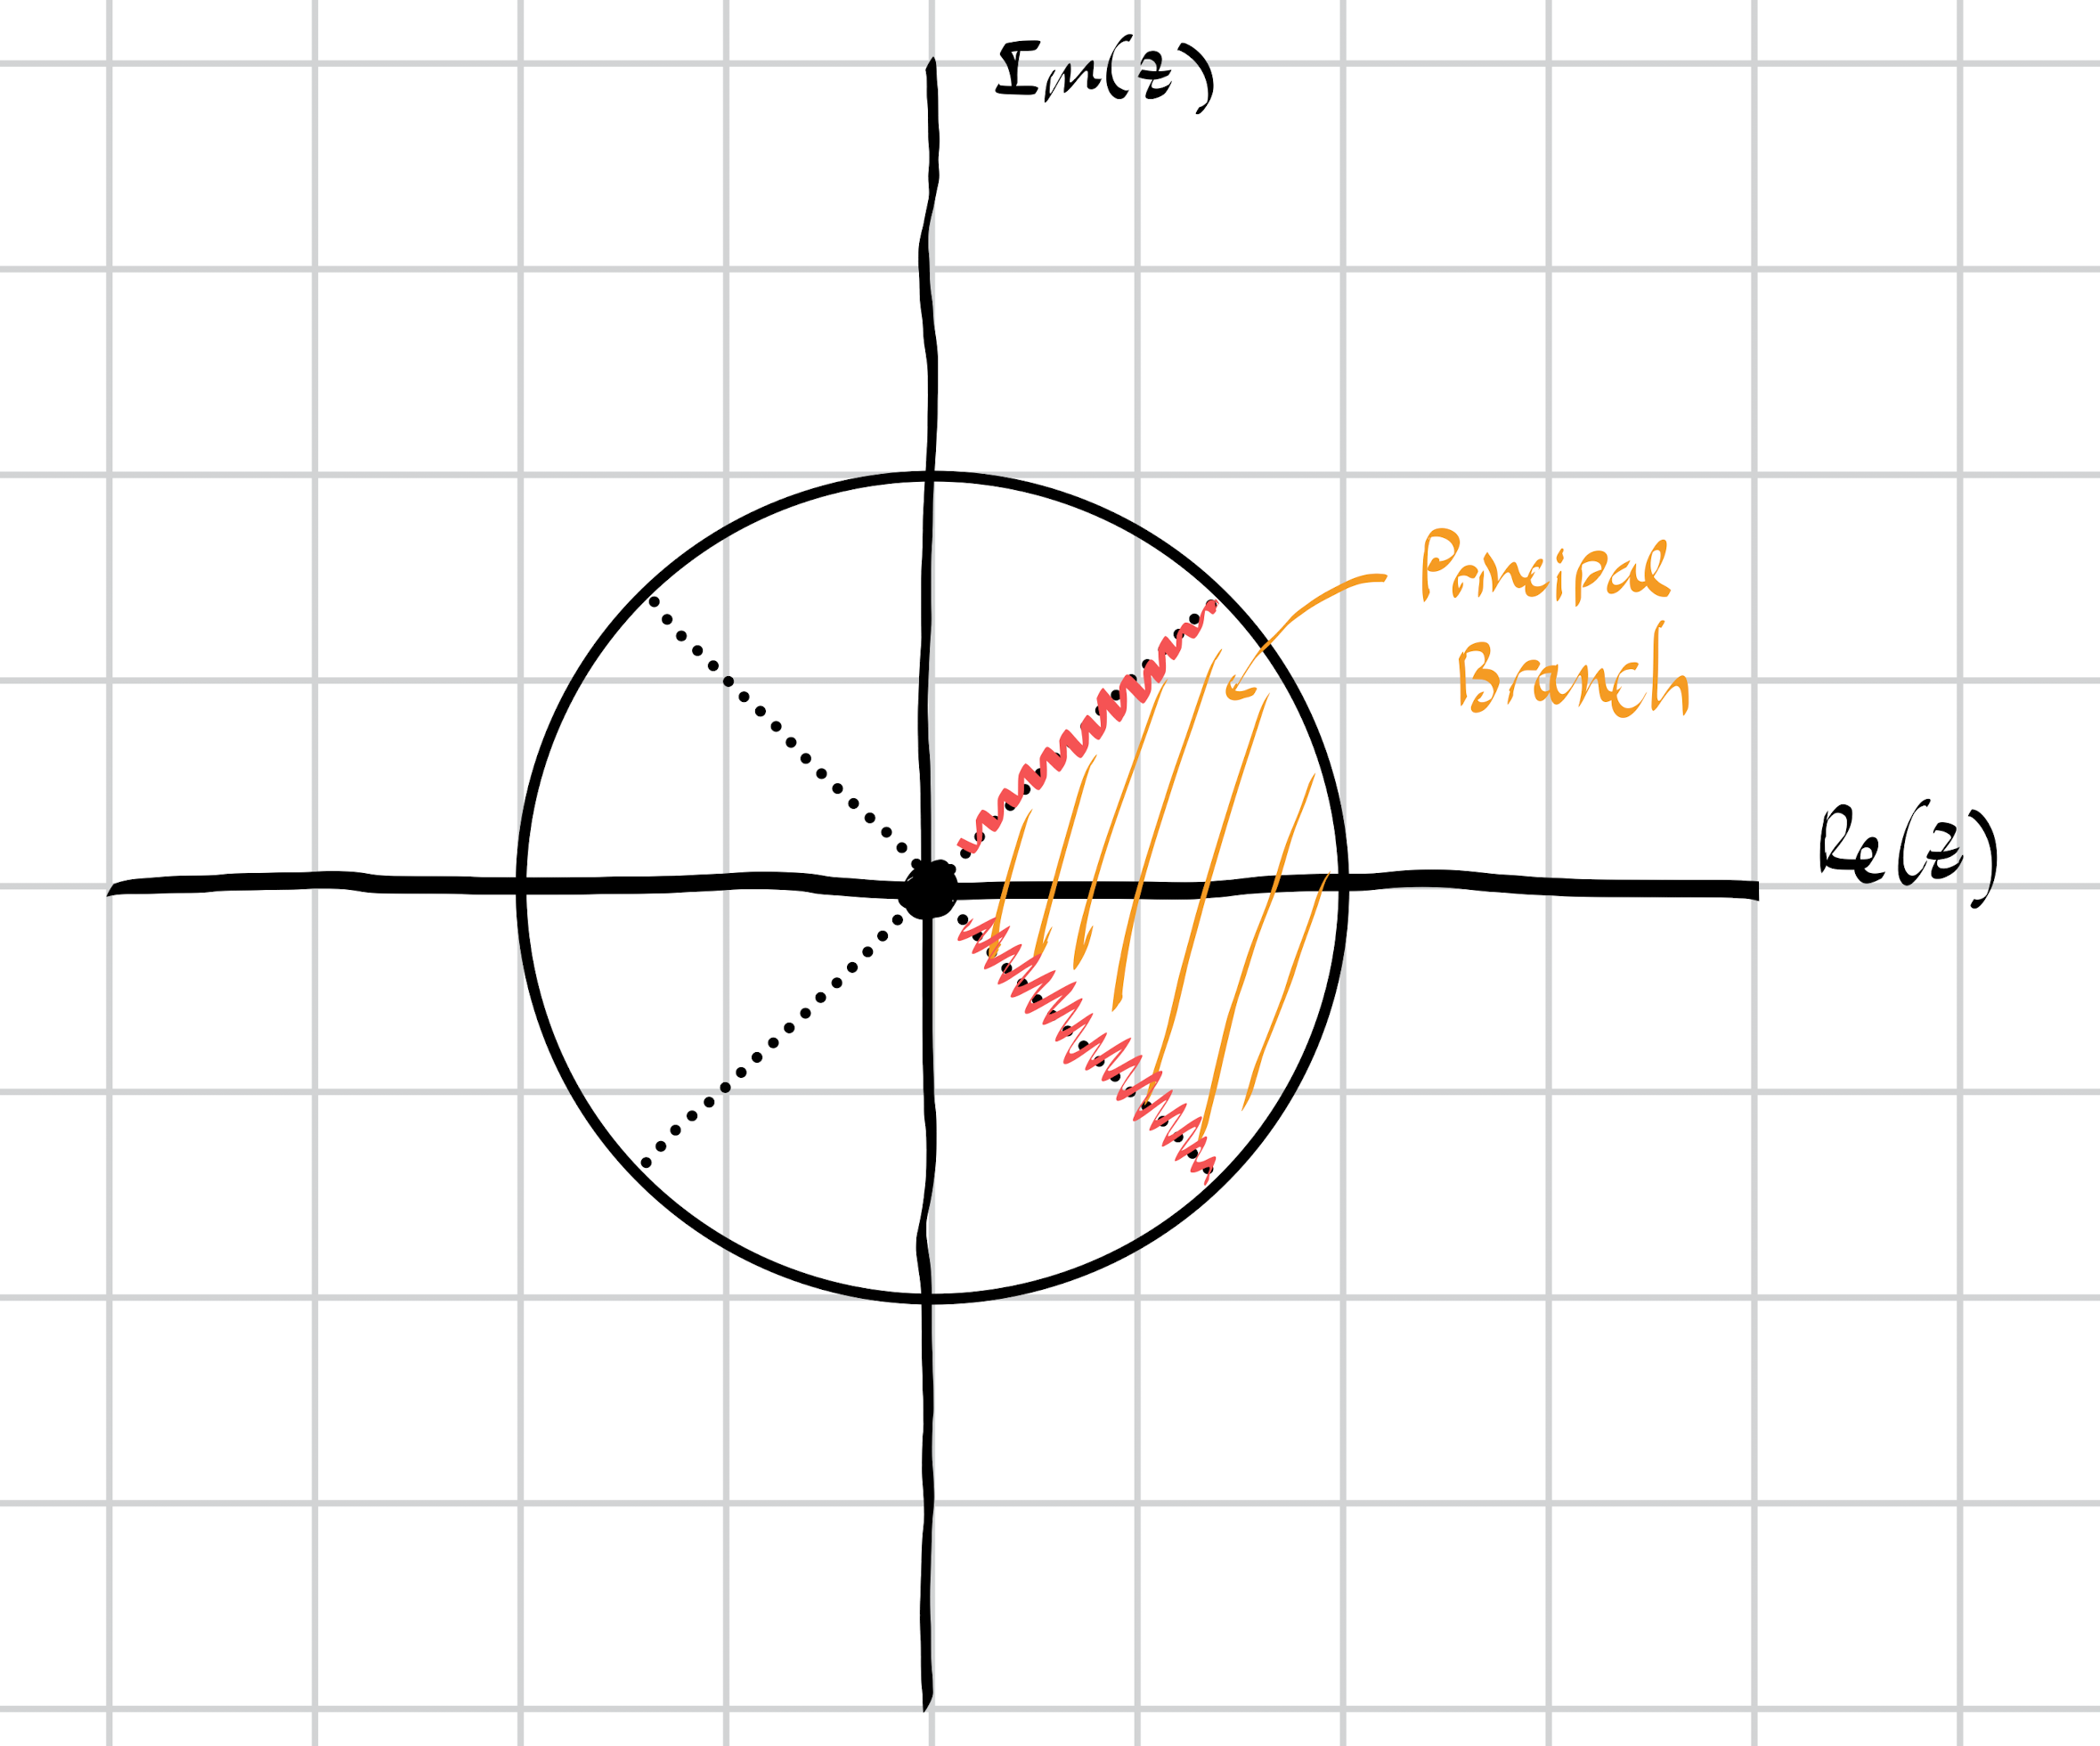
\includegraphics[width=10cm]{images/19_11.png}
  \end{center}
\end{solution}
\begin{solution}[19.13]
  Writing
  \begin{align*}
    \sqrt{z^2 + 1} &= \sqrt{\left( z-i \right)\left( z+i \right)},
  \end{align*}
  we look at the contours $\pm i$. Define
  \begin{align*}
    z_{\pm} &= \left( z\mp i \right)\\
            &= r_{\pm}e^{i\varphi_{\pm}}.
  \end{align*}
  Plugging into our expression, we get
  \begin{align*}
    w(z) &= \sqrt{r_{+}r_{-}}e^{i\left( \varphi_{+} + \varphi_{-} \right)/2}.
  \end{align*}
  If we go around the contour at $z = i$, then $\varphi_{+}$ will rotate around by $2\pi$, while $\varphi_{-}$ will not rotate around by $2\pi$. Similarly, if we go around the contour at $z = -i$, then $\varphi_{-}$ will rotate around by $2\pi$ while $\varphi_{+}$ will not rotate around by $2\pi$.\newline

  Meanwhile, if we have the contour around both $z=i$ and $z = -i$, then both $\varphi_{+}$ and $\varphi_{-}$ rotate around by $2\pi$, meaning we do not pick up a sign change.\newline

  We take the branch cut between $z = i$ and $z = -i$ to allow contours that circle both $z = \pm i$ but disallow contours that only circle one of $z = \pm i$.
\end{solution}
\begin{solution}[19.18]\hfill
  \begin{enumerate}[(a)]
    \item Consider
      \begin{align*}
        w(1/\zeta) &= \sqrt{\left( \frac{1}{\zeta}-a_1 \right) \cdots \left( \frac{1}{\zeta}-a_n \right)}\\
               &= \frac{1}{\zeta^{n/2}}\sqrt{\left( 1-a_1\zeta \right)\cdots \left( 1-a_n \zeta \right)}.
      \end{align*}
      We have a branch point at $\zeta = 0$ whenever $n/2\notin \Z$, as then it is the case that the square root has multivalued behavior.
    \item Considering
      \begin{align*}
        w\left( 1/\zeta \right) &= \sqrt{1/\zeta - a_1} + \cdots + \sqrt{1/\zeta - a_n}\\
                                &= \frac{1}{\zeta^{1/2}}\sqrt{1-a_1\zeta} + \cdots + \frac{1}{\zeta^{1/2}}\sqrt{1-a_n\zeta},
      \end{align*}
      we see that each $\zeta^{1/2}$ has branching behavior as $ \zeta\rightarrow 0 $, so $w$ has a branch point at $\infty$.
  \end{enumerate}
\end{solution}
\begin{solution}[19.24]
  We must move $e^{2\pi i}$ back into the principal branch to evaluate the square root.
\end{solution}
\begin{solution}[19.28]\hfill
  \begin{enumerate}[(a)]
    \item We have
      \begin{align*}
        e^{iz} &= \cos(z) + i\sin(z)\\
               &= \left( 1-\sin^2(z) \right)^{1/2} + i\sin(z).
      \end{align*}
      Thus, defining $w = \sin(z)$, we have
      \begin{align*}
        iz &= \ln\left( iw + \left( 1- w^2\right)^{1/2} \right)\\
        z &= -i\ln\left( iw + \left( 1-w^2 \right)^{1/2} \right).
      \end{align*}
      Similarly, defining $w = \cos(z)$, we have
      \begin{align*}
        e^{iz} &= \cos(z) + i\left( 1-\cos^2(z) \right)^{1/2}\\
        iz &= \ln\left( w + i\left( 1-w^2 \right)^{1/2} \right)\\
           &= \ln\left( w + i\left( \left( -1 \right)\left( w^2 - 1 \right) \right)^{1/2} \right)\\
           &= \ln\left( w + i\left( -i \right)\left( w^2 - 1 \right)^{1/2} \right)\\
           &= \ln\left( w + \left( w^2 - 1 \right)^{1/2} \right).
      \end{align*}
    \item The principal branch of $\ln$ gives outputs in the range $(-\pi,\pi)$. 
  \end{enumerate}
\end{solution}

\end{document}
